%======================================================================
\chapter{Measuring Renyi Entanglement Entropy}
%======================================================================
\comment{Totally why do we measure this?  Y'know?}\\
\comment{Mention we're using double projector}

\noindent
- we can't measure \vn with vb qmc\\
- \vb isn't a good measure of entropy\\
- can measure \re\\
 - closest entropy to \vn\\
 - gives a lower bound on \vn\\
 - maybe follows same area law and still has universal terms? (check)\\
 
The generalized Renyi entanglement entropies, again defined as:
\begin{equation} \label{renyi2}
 	S_n(\rho_{\rm A}) = \frac{1}{1-n}\ln\left[{\rm Tr}\left( \rho_{\rm A}^n \right) \right],
\end{equation}
where $\rho_{\rm{A}}=\rm{Tr}_B\ket{\psi}\bra{\psi}$ is the reduced density matrix of region A, and $n>0$.

\change{
``Encode information about the whole entanglement spectrum of $\rho_{\rm A}$."
(But that's just because if you know all of them you pretty much know all the eigenvalues of $\rho_{\rm A}$.)
So they have more information together than just $S_1=\VN$. \cite{Spectrum}
}

\change{ Something about topological entanglement entropy and quantum dimension \cite{Bbob}.}

\change{ Field theory on $O(N)$ model... universal corrections to scaling of $S_n$ calculated.}

The Renyi entropies have the property that successive entropies give a lower bound on the previous entropies.  I.e. if $n>m$ then $S_n<S_m$, so \re gives a lower bound on \vN, and \re will give the closest estimate of \vN.

We can use the expectation value of a unitary \sw operator on two non-interacting copies of the system to be studied in order to obtain ${\rm Tr}(\rho_{\rm A}^2)$, a quantity necessary to compute \re.  
This process can be generalized to calculate any $S_n$ with $n \ge 2$, by applying a generalized \sw operator to $n$ copies of the system. 

\section{The ``Replica Trick''}
%----------------------------------------------------------------------------------------------------------
\subsection{The Swap Operator}
%----------------------------------------------------------------------------------------------------------

\begin{figure} {
	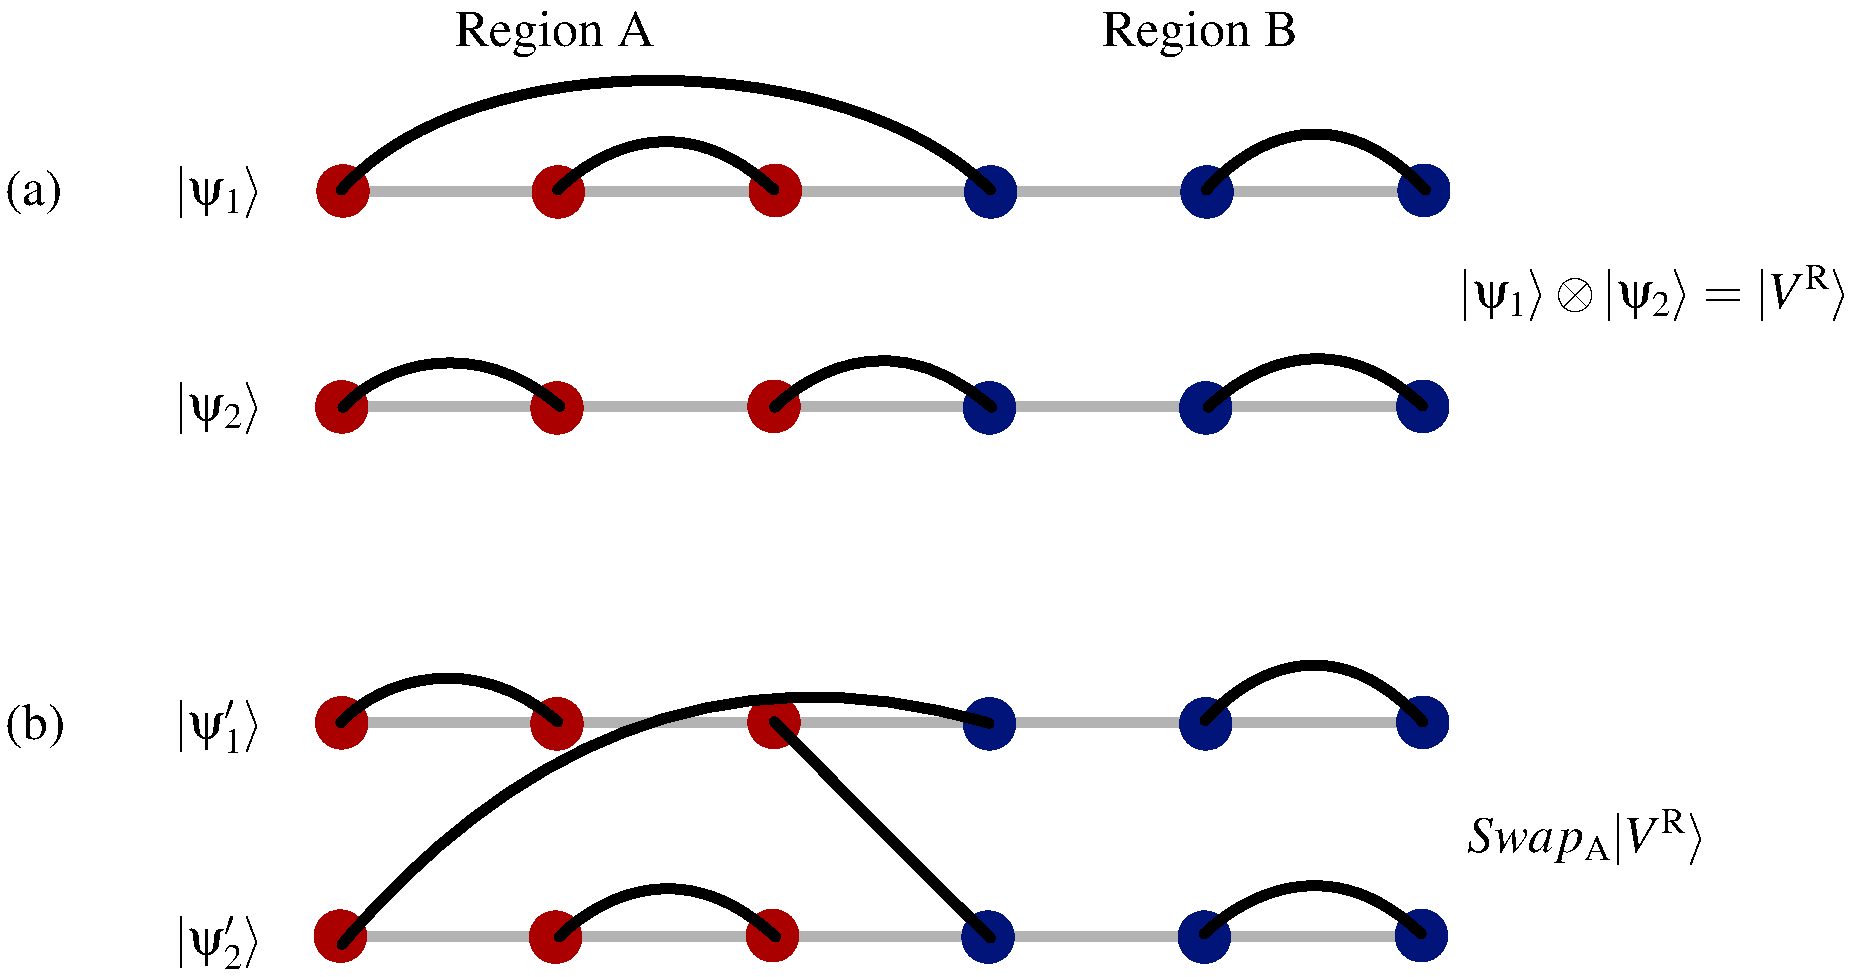
\includegraphics[width=6.2 in]{./figures/made/swp.pdf} 
	\caption[Application of the Swap operator]{
		\label{swap}
		(a) Two non-interacting copies, $\ket{\psi_1}$ and  $\ket{\psi_2}$, of a six-site chain
		where the left three sites of each copy belong to region A, and the other sites are in
		region B.
		
		(b) The same system from (a) after the $Swap_{\rm A}$ operator is applied.
		The endpoints of the valence bonds in region A are switched between copies 
		of the system.  Region B remains unswapped.
	}
}\end{figure}

The \swa operator acts on two copies of the system (see Figure \ref{swap}), where the copies are not necessarily in the same state.  The action of \swa is to exchange the configuration of region A, between the two copies of the system.  If region A has some entanglement with region B in one of both of the copies of the system, then the two copies will become entangled after the application of \swA.
The \swa operator can be more clearly defined in a basis such as the $S^z$ basis, in which an arbitrary state can be represented as a weighted sum of states decomposed into the separate a region A and a region B configuration.  
If we define $\{\ket{\alpha}\}$ as a complete basis of states spanning region A, and $\{\ket{\beta}\}$ as a complete basis of states spanning region B, then we can represent an arbitrary state as
\begin{equation}
	\ket{\psi} = \sum_{\alpha}\sum_{\beta} C_{\alpha,\beta}\ket{\alpha}\ket{\beta}
\end{equation}
for some set of coefficients $C_{\alpha,\beta}$.  
Then the effect of \swa on a two general states, $\ket{\psi_1}$ and $\ket{\psi_2}$ representing the two copies of the system, is
\begin{align}
	\SWA \ket{\psi_1} \otimes \ket{\psi_2}  &= 
		\SWA \left(\sum_{\alpha_1,\beta_1} 
		C_{\alpha_1,\beta_1}\ket{\alpha_1}\ket{\beta_1}\right) \otimes
			\left(\sum_{\alpha_2,\beta_2} 
		C_{\alpha_2,\beta_2}\ket{\alpha_2}\ket{\beta_2}\right) \\
			&=\sum_{\alpha_1,\beta_1}C_{\alpha_1,\beta_1}\sum_{\alpha_2,\beta_2} 
			C_{\alpha_2,\beta_2}
			\big(\ket{\alpha_2}\ket{\beta_1}\big)\otimes\big(\ket{\alpha_1}\ket{\beta_2}\big).
\end{align}
And the expectation value of \swa acting on two non-interacting copies of the ground state will be
\begin{align}
\langle \SWA \rangle &=
\bra{\Psi_0\otimes\Psi_0}\SWA \ket{\Psi_0\otimes\Psi_0} \\ 
	&=\sum_{\alpha_1,\beta_1} \sum_{\alpha_2,\beta_2}
		\overline{C}_{\alpha_2,\beta_1}C_{\alpha_1,\beta_1}
		\overline{C}_{\alpha_1,\beta_2}C_{\alpha_2,\beta_2}\\
	&=\sum_{\alpha_1,\alpha_2} \bra{\alpha_1}\rho_{\rm A} \ket{\alpha_2} 
					\bra{\alpha_2}\rho_{\rm A} \ket{\alpha_1}\\
	&={\rm Tr (\rho_A^2)}.
\end{align}
For more detail see Appendix \ref{swaperator}.  From Equation \eqref{renyi} the second Renyi entanglement entropy is
\begin{equation}
	S_2(\rho_{\rm A}) = -\ln\!\left[{\rm Tr}(\rho_{\rm A}^2)\right] = -\ln\left( \langle \SWA \rangle \right), \label{swapspectation}
\end{equation}
independent of basis.  Specifically, we can use \eqref{swapspectation} in the valence bond basis, where the \swa operator acts to swap the endpoints of valence bonds within region A between copies of the system, as in Figure \ref{swap}.

%----------------------------------------------------------------------------------------------------------
\subsection{Measuring the Swap Operator}
%----------------------------------------------------------------------------------------------------------

Since we are using the double projector algorithm for these measurements (Section \ref{sec:dubproj}) we use equations \eqref{generalop1} and \eqref{generalop2} to measure the \swa operator,
\begin{equation}
\langle \SWA \rangle = 
 \frac{   \sum_{l,r} W^L_l W^R_r  \bra{V^L_l} V^R_r\rangle    
		\frac{   \bra{V^L_l} \SWA  \ket{V^R_r}  }{   \bra{V^L_l} V^R_r\rangle  }}
							{\sum_{l,r} W^L_l W_r^R \bra{V^L_l} V^R_r\rangle}
	= \left<
		\frac{   \bra{V^L} \SWA \ket{V^R}  }{   \bra{V^L} V^R\rangle  }
						\right>,
\label{swapmeas}
\end{equation}
though in this case $\ket{V^{\rm L}}$ and $\ket{V^{\rm R}}$ each contain two non-interacting copies of the system we want to study, depicted in Fig.~\ref{swap}.


%----------------------------------------------------------------------------------------------------------
\section{1D Results}
%----------------------------------------------------------------------------------------------------------
\begin{figure} {
	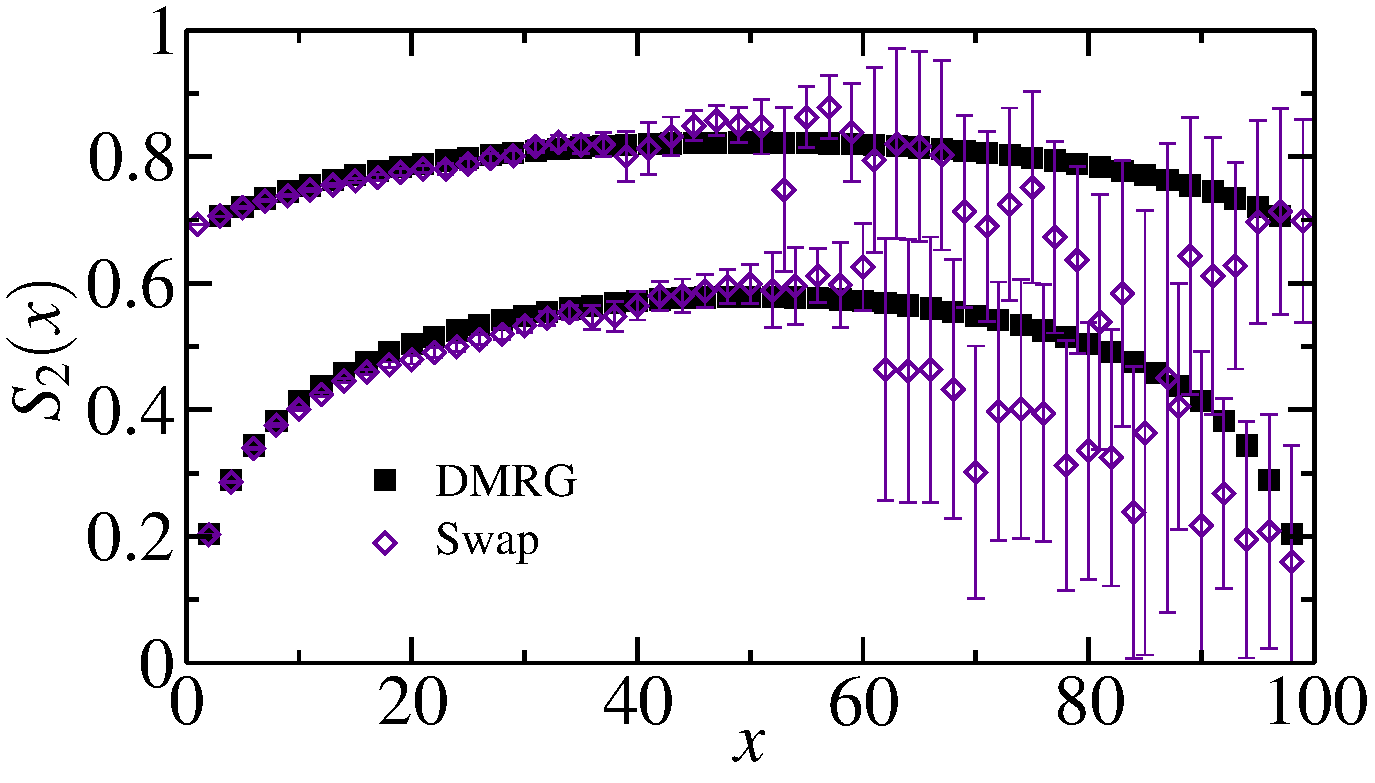
\includegraphics[width=6in]{./figures/paper2/fig_1D/swapfig.pdf} 
	\caption[Renyi for 100 site chain]{ 
	\label{swapfig}
	The Renyi entropy $S_2$ as a function of site index $x \in $ A, for a 100-site Heisenberg chain with open boundaries, 
		calculated with DMRG and VB QMC.  Data labeled ``Swap'' was calculated with Eq.~\eqref{swapmeas} with one VB QMC simulation.	
	}
}\end{figure}

We begin by measuring $S_2$ for a 1D OBC chain of length $L=100$, using the expectation value of the $Swap_x$ operator to find $S_2$ in VB QMC, where sites 1 through $x$ are included in region A. 
The trial state $\ket{V}$ used is a simple dimerized state with only nearest neighbor valence bonds.
Results are shown in Figure \ref{swapfig}.
In the DMRG simulations, $S_2$ is calculated in the standard way, using the eigenvalues of the reduced density matrix. 
One can immediately see that the calculation of $S_2$ with the expectation value $\langle \SWA \rangle$ gives very large statistical errors, especially for a large number of sites inside region A.

One way to understand to consider what we are actually measuring.
From Eq. \eqref{swapmeas} one can see we are measuring the ratio of two inner products.
Since the overlap (Eq. \eqref{innprod}) is $2^{N_{\rm loop} - N_{\rm sites}/2}$, this ratio of inner products is $2^{N_{\rm swaploops} - N_{\rm loops}}$.
The quantity we measure depends entirely of the change in the number of loops after applying a swap operator to one of our states. 
For a large region A we are swapping a larger number of sites, and the difference in the number of loops can change by a large number, or a small number. 
We have to sample states for much longer to converge on the average change in the number of loops.
In contrast, swapping only one site ($x=1$) will always decrease the number of loops by 1, so $S_2(1)=\ln(2)$ always.
For two sites in region A, the difference in the number of loops can be $-2$ or 0. \comment{Check the numbers, and maybe extend or find a formula.} 
\comment{Cram some diagrams of this up in here.}
\change{
Another way to look at it is that we are sampling terms in the trace of a much larger matrix for a large region A.}

One way to improve upon the poor sampling of  $\langle \SWA \rangle$ is using the loop algorithm (Section \ref{sec:loop}), which \change{has much better scaling?} than the double projector method.
Measurements taken using the loop algorithm are added into Figure \ref{loopfig}; they show a significant improvement over the double projector $\langle \SWA \rangle$ measurement, 
though there is still noticeable statistical error for large region A.
If our goal was simply the measurement of $S_2$ instead of the demonstration of the most effective way to measure $S_2$, we could note that $S_2(A) = S_2(B)$ and reflect the data about the midpoint, resulting in almost perfect correspondence with the DMRG data.
However, when we begin to measure larger system sizes and move to 2D the deficiencies in measuring the bare \swa operator will become increasingly apparent; it is necessary to improve upon this measurement technique, which we have done using an ``improved ratio'' sampling scheme.




\begin{figure} {
	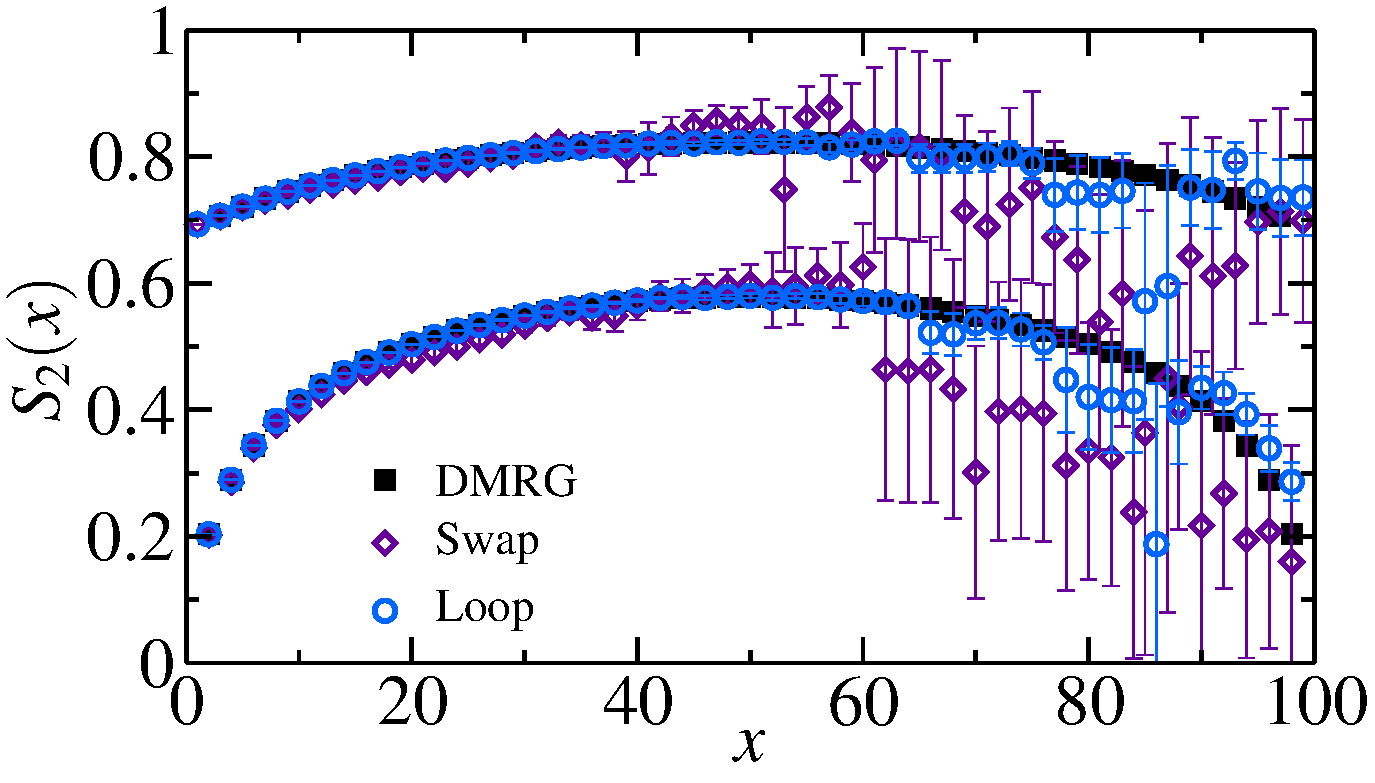
\includegraphics[width=6in]{./figures/paper2/fig_1D/loopfig.pdf} 
	\caption[Renyi for 100 site chain with loop algorithm data]{ 
	\label{loopfig}
The Renyi entropy $S_2$ as a function of site index $x \in $ A, for a 100-site Heisenberg chain with open boundaries, 
calculated with DMRG, VB QMC double projector algorithm (labelled Swap), and the VB QMC loop algorithm (labelled Loop).
}
}\end{figure}


	

%----------------------------------------------------------------------------------------------------------
\section{``Improved Ratio'' Sampling}
%----------------------------------------------------------------------------------------------------------


\begin{figure} {
	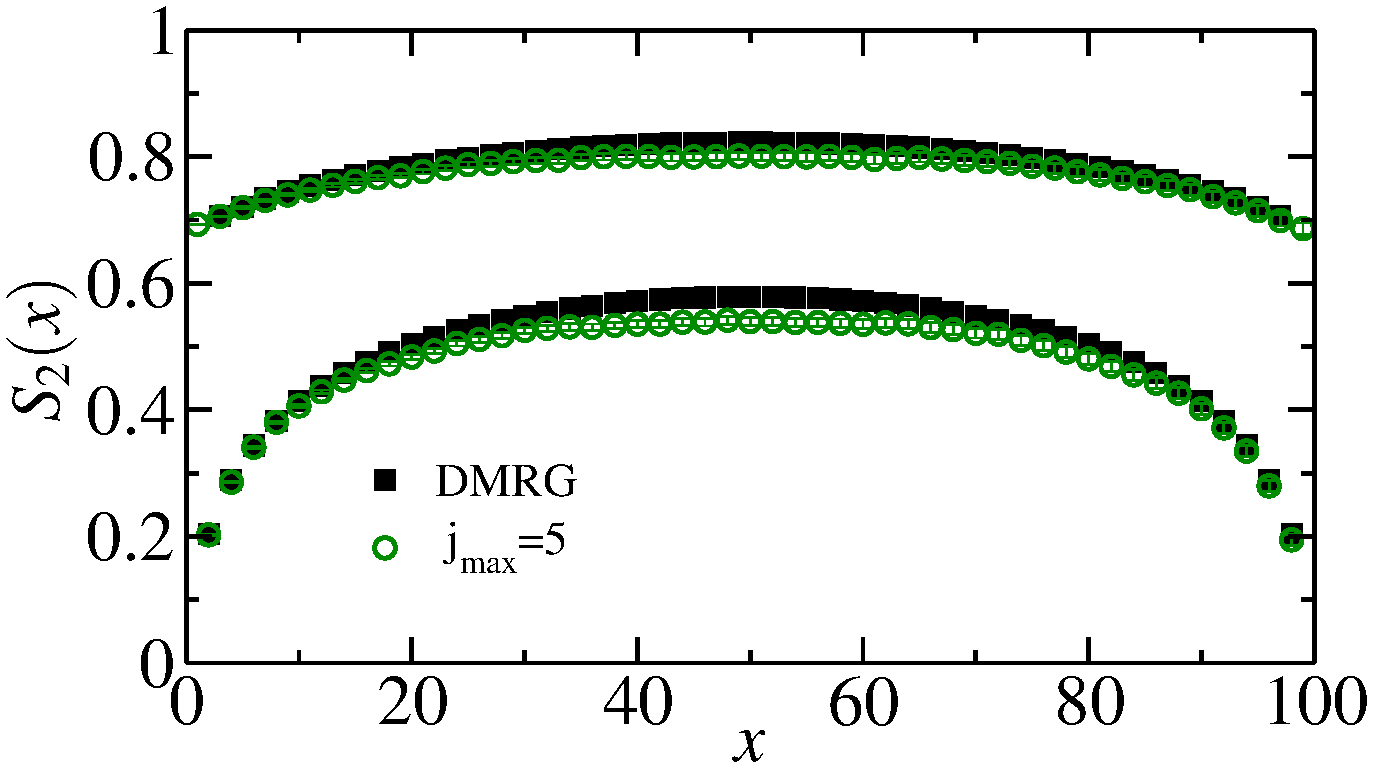
\includegraphics[width=6in]{./figures/paper2/fig_1D/ratiofig.pdf} 
	\centering
	\caption[Renyi for 100 site chain with ratio data]{ 
	\label{ratiofig}
	DMRG and improved ratio data for a 100-site Heisenberg chain with open boundaries.
The ratio data uses $j_{\rm max}=5$ and required 20 separate simulations.
	}
}\end{figure}

Instead of measuring  $\langle Swap_x \rangle$ for a region A including $x$ sites, we measure a ratio of different $Swap_x$ operators,
\begin{equation}
\label{eqratio}
\frac{\langle Swap_{x+j}\rangle}{\langle Swap_{x}\rangle} = 
\frac{ \sum_{l,r} W^L_l W^R_r \bra{V^L_l}Swap_{x+j} \ket{V^R_r}}
							{\sum_{l,r} W^L_l W_r^R \bra{V^L_l} Swap_x \ket{ V^R_r}},
\end{equation}
where $j=1,\dots,j_{\rm max}$ is the difference between the region sizes for the two $Swap$ operators.
To get to the entanglement entropy from here we take the negative logarithm of \eqref{eqratio} to get
\begin{equation}
\label{eqratio2}
-\ln\left( \frac{\langle Swap_{x+j}\rangle}{\langle Swap_{x}\rangle} \right) = 
-\ln \langle Swap_{x+j}\rangle + \ln\langle Swap_{x}\rangle   =   S_2(x+j) - S_2(x),
\end{equation}
so we can extract $S_2(x+j)$ if we have $S_2(x)$ from a previous measurement.
The sampling weight from \eqref{supaweight} is modified with this new measurement, to be
\begin{equation}
W_{\rm total} = W^LW^R\bra{V^L} Swap_x \ket{V^R}.
\end{equation}
However, modifying the sampling weight in this way means we can only measure the ratio \eqref{eqratio} for one value of $x$ per simulation.
To get $S_2$ for all region sizes we first choose a value for $j_{\rm max}$.
A small $j_{\rm max}$ means more improvement due to the ratio, but also more simulations are required.
We then measure the bare $\langle Swap_{j}\rangle$ for $j=1,\dots,j_{\rm max}$ in our first simulation.
The second simulation measures the ratio $\langle Swap_{x+j}\rangle / \langle Swap_{x}\rangle$ with $x=j_{\rm max}$.  The following simulations use $x=2j_{\rm max}, 3j_{\rm max}, 4j_{\rm max}, \dots$ until we reach the maximum size of region A.
The number of simulations need for a 1D system is $(L/j_{\rm max})$.

Figure \ref{ratiofig} shows the ratio data using $j_{\rm max} = 5$, along with the DMRG data, for the same 100-site system as in Figs. \ref{loopfig} and \ref{swapfig}. 
The data no longer show the large statistical error bars for large region A sizes, though the results are systematically lower than the DMRG $S_2$ results for a region A-B boundary near the middle of the 100-site system.  
This can be improved by choosing a smaller value of $j_{\rm max}$.



%----------------------------------------------------------------------------------------------------------
\section{2D Results}
%----------------------------------------------------------------------------------------------------------

\begin{figure} {
	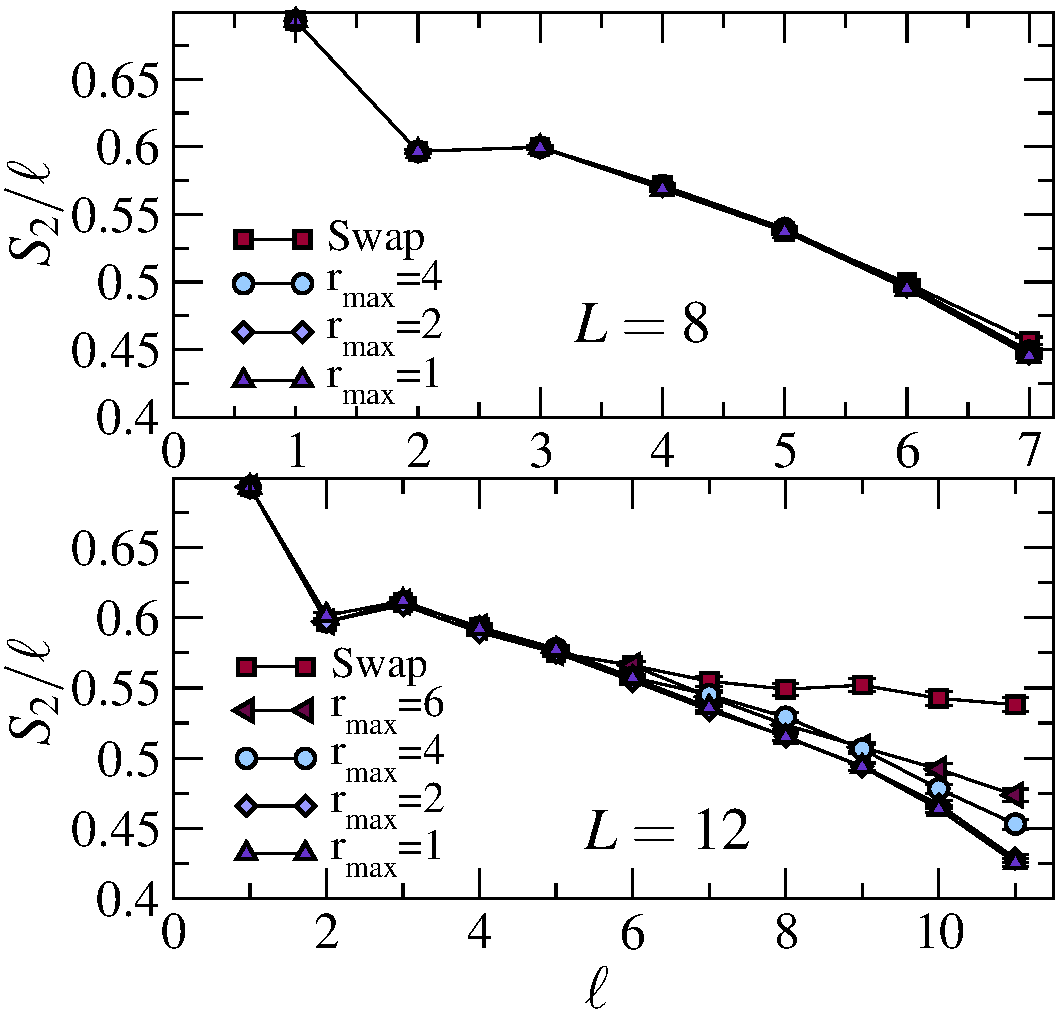
\includegraphics[width=6in]{./figures/paper2/fig_2DA/L8n12_ratio.pdf} 
	\caption[$S_2$ in an $8 \times 8$ and $12 \times 12$ system]{ 
	Measurements of $S_2/\ell$ for $8 \times 8$ and $12 \times 12$ PBC systems with a region A of size $\ell \time \ell$.
	The bare $\langle Swap_\ell \rangle$ results are shown along with the improved ratio results for different values of $r_{\rm max}$.
	\label{2Dfig}
	}
} \end{figure}

We now look at 2D $L\times L$ systems with PBC, where region A is an $\ell \times \ell$ and region B is the remainder of the system.
For this system we must slightly change the definition of our improved ratio estimator to fit the different geometry.
Instead of $j$ and $j_{\rm max}$ from \eqref{eqratio} and \eqref{eqratio2} we now use $r$ and $r_{\rm max}$, and measure $\langle Swap_{\ell+r}\rangle / \langle Swap_{\ell}\rangle$ where $\ell +r$ is the linear dimension of a square region A, and $r=1,\dots,r_{\rm max}$.
We increase the size of region A such that it is always a square, adding a row and column of sites simultaneously.

Figure \ref{2Dfig} shows the $Swap$ and ratio results for 2D PBC systems of size $8 \times 8$ and $12 \times 12$.
For the $8\times 8$ system the results are already almost entirely converged with the $Swap$ measurement, and the ratio measurements only offer a very slight improvement.
	When the system size is increased to $12 \times 12$ the ratio results significantly improve the measurement, though the $r_{\max} = 2$ and $r_{\max} = 1$ results almost exactly overlap, implying that the results have converged to the correct answer at that point.
	It is possible to improve the sampling even further adding one site at a time to the region size, instead of only increasing the linear dimension of region A.
	We should note that for large values of $r_{\rm max}$ the correct value of $S_2$ does not fall within the error bars of the data, indicating that the low sampling of the $Swap$ operator may weaken the ergodicity of the simulation.

%----------------------------------------------------------------------------------------------------------
\section{The Area Law}
%----------------------------------------------------------------------------------------------------------

\begin{figure} {
	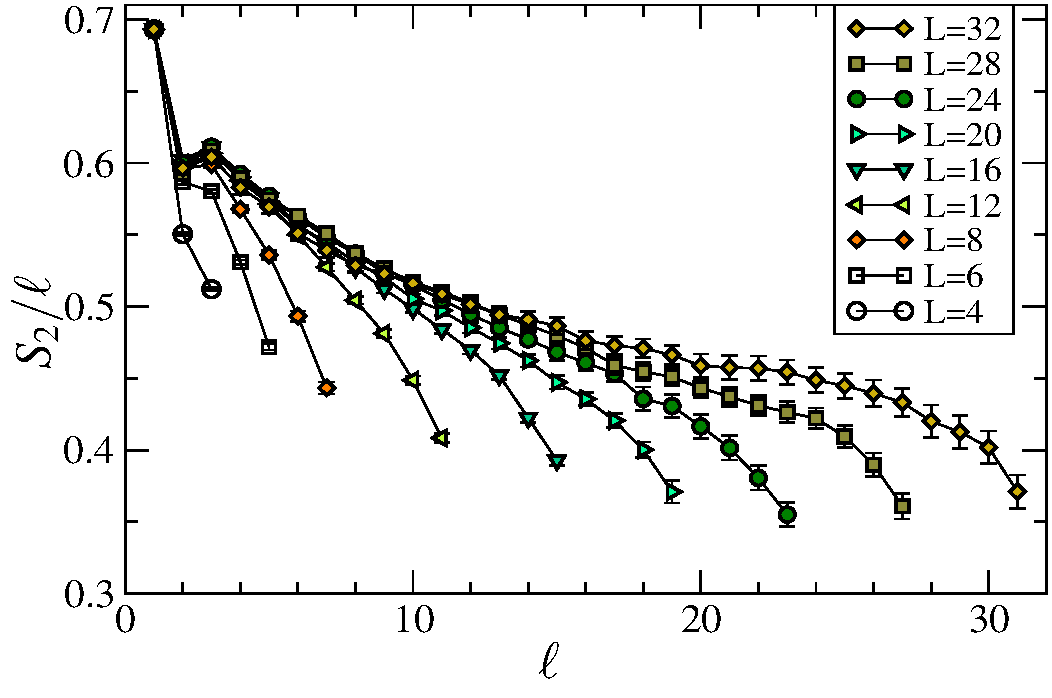
\includegraphics[width=5in]{./figures/paper2/fig_AreaL/fig4.pdf} 
	\centering
	\caption[Area law for $S_2$ in the N\'eel state]{
Scaling of the entanglement entropy $S_2/\ell$ plotted for versus $\ell$ for different sizes of the $\ell \times \ell$ region A and different $L \times L$ system sizes. 
The data are calculated using the 2D improved ratio estimator \comment{eqref} with $r_{\rm max} = 1$.
	\label{2Darea}
	}
} \end{figure}

Using the improved ratio estimator we now examine larger regions of the same geometry as used in the previous section (PBC $L \times L$ systems with an $\ell \times\ell$ region A) in an attempt to extract area law scaling of the entanglement entropy.
Figure \ref{2Darea} show $S_2/\ell$ results for systems from $L=4$ to $L=32$.
From Section \ref{vbAlaw} and Ref. \cite{PRL1} one expects the scaling of $S_1 = \VN$ in the N\'eel state to follow the area law, and from \comment{some equation} we know that $S_2 \le \VN$.
The data in Fig. \ref{2Darea} appears consistent with the area law $S_2/\ell \sim \text{const.}$ for $\ell \ll L$, in particular we do not see a multiplicative log correction that was present in the scaling of \vb \cite{Alet, Chh}. 

Next we examine entanglement entropy scaling for the ladder geometry studied in Section \ref{vbAlaw} and Ref. \cite{PRL1}.
The results are shown in Figure \ref{2Dbetter1}, including both DMRG and ratio estimator VB QMC data.  
From the DMRG data alone it is not immediately apparent that $S_2/M \sim$ const., especially considering the trend in the first few data points. 
Fortunately, the range system sizes we can study is extended by the \swa measurement with VB QMC, and the added points make it clear that $S_2$ does in fact follow an area law for the N\'eel state.

In Figure \ref{2Dbetter2} we examine the same systems with only $M^2$ sites in region A.
For the small system sizes we see much larger even-odd oscillations, as we go to larger system sizes both Figs. \ref{2Dbetter1} and \ref{2Dbetter2} follow the same area law scaling.


\begin{figure} {
	\hspace{1cm}
	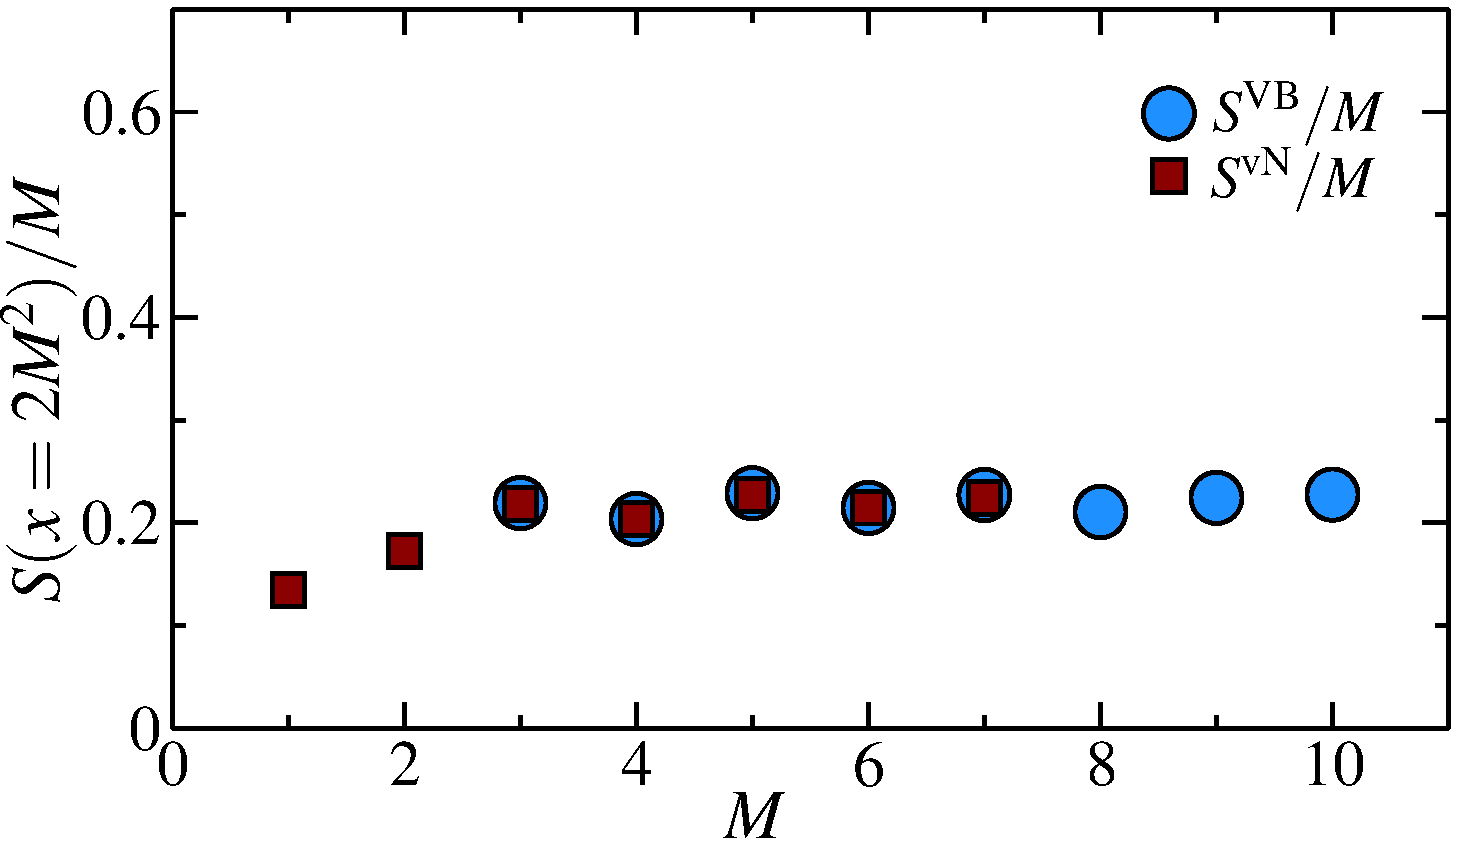
\includegraphics[width=5in]{./figures/made/awesomeplot/marea2.pdf} 
	\caption[fds]{ 
Scaling of the entanglement entropy $S_2/M$ plotted for versus $M$, for $M$-leg ladders of length $4M$.  
Region A contains $2M^2$ sites, dividing the ladders in half with the cut is across the $M$ legs, using one of the same geometries as is found in Fig. \ref{zigzag}.
The data were measured using the 2D improved ratio estimator using $j_{\rm max} = M$.
	\label{2Dbetter1}
	}
} \end{figure}
\begin{figure} {
\hspace{1cm}
	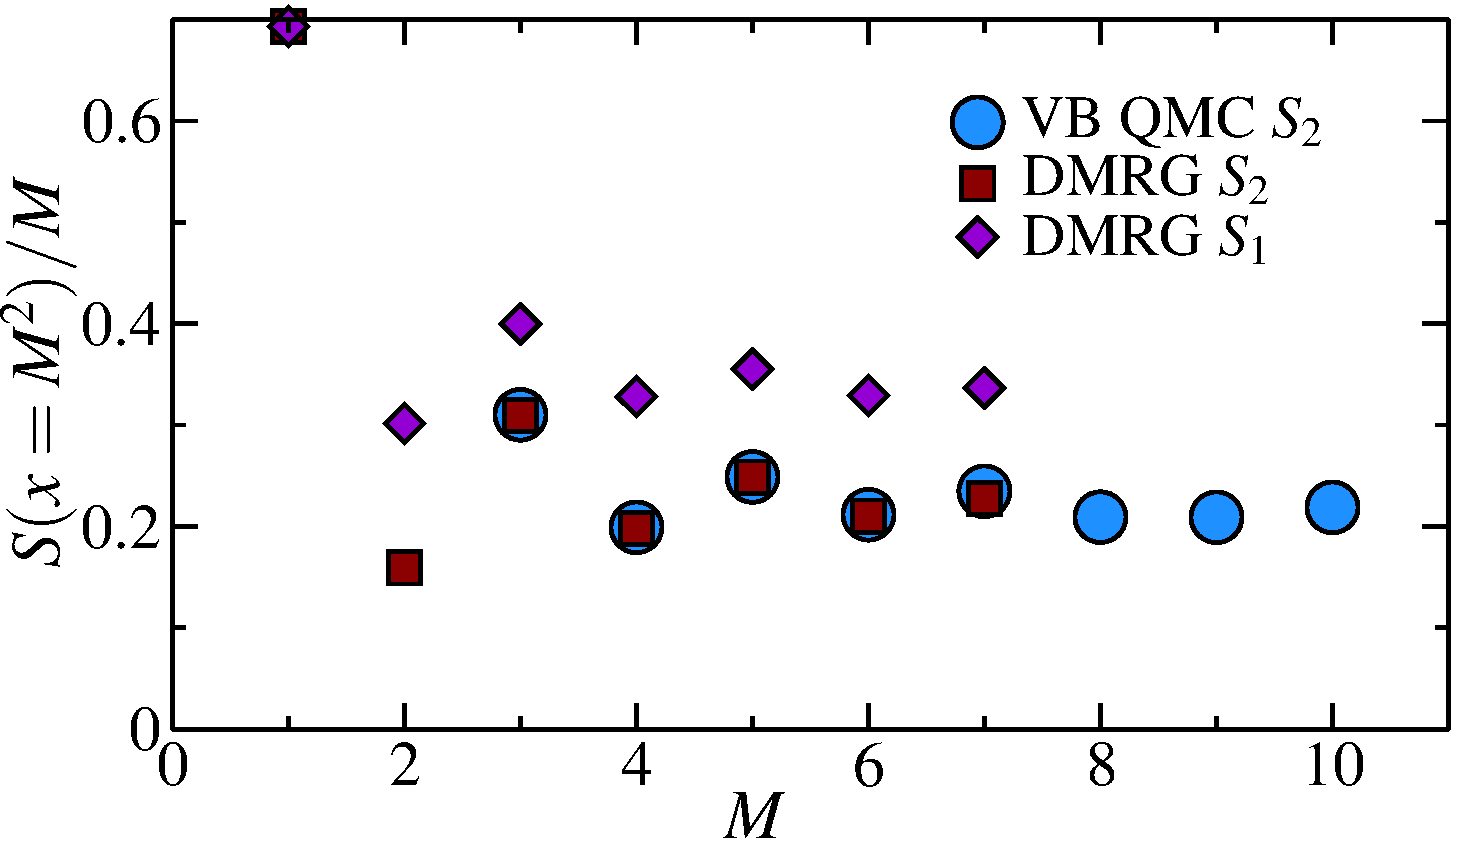
\includegraphics[width=5in]{./figures/made/awesomeplot/marea.pdf} 
	\caption[fds]{ 
	Scaling of the entanglement entropy $S_2/M$ plotted for versus $M$, for $M$-leg ladders of length $4M$.  
Region A contains $M^2$ sites, dividing the ladders into segments one-quarter and three-quarters of its length, where cut is across the $M$ legs.  This geometry is quite similar to one of the geometries used in Fig \ref{zigzag}.
The data were measured using the 2D improved ratio estimator using $j_{\rm max} = M$.
		\label{2Dbetter2}
	}
} \end{figure}

%----------------------------------------------------------------------------------------------------------
\section{Conclusions}
%----------------------------------------------------------------------------------------------------------
